% ============================================================================
% CHAPITRE 3 — SPRINT 1 : MISE EN PLACE DE L'ENVIRONNEMENT ET INTERFACE
% ============================================================================

\section{Introduction}

Ce chapitre détaille le déroulement du Sprint~1 du projet Guidni. Ce premier Sprint, d'une
durée de quatre semaines (octobre 2024), est consacré à la mise en place de l'environnement
de développement, à la définition de l'architecture de base et à la préparation de l'interface
utilisateur. Pour cela, j'ai suivi le plan suivant~:
\begin{enumerate}
    \item Planning du Sprint
    \item Analyse
    \item Conception
    \item Réalisation
    \item Sprint Review
\end{enumerate}


% ────────────────────────────────────────────────────────────────
\section{Planning du Sprint~1}
% ────────────────────────────────────────────────────────────────

\subsection{Objectif du Sprint}

L'objectif du Sprint~1 est d'asseoir les fondations conceptuelles et architecturales du système
Guidni. La complexité inhérente à l'hybridation d'un agent cognitif et d'un algorithme
d'apprentissage par renforcement impose une définition rigoureuse des flux de données avant
toute implémentation. Les livrables attendus sont les artefacts documentaires, les diagrammes
de spécification technique et l'environnement de développement opérationnel.

\subsection{Sprint Backlog}

\begin{table}[H]
    \centering
    \caption{Sprint Backlog --- Sprint~1}
    \label{tab:sprint1_backlog}
    \small
    \begin{tabular}{c c p{7cm} c}
        \toprule
        \textbf{ID US} & \textbf{ID Task} & \textbf{Task} & \textbf{Complexité} \\
        \midrule
        US-01 & T-1.1 & Configuration de l'environnement Python 3.12 et FastAPI & S \\[3pt]
        US-01 & T-1.2 & Installation et configuration de PostgreSQL 15 & S \\[3pt]
        US-01 & T-1.3 & Configuration du serveur Ollama avec qwen2.5:7b & M \\[3pt]
        US-02 & T-1.4 & Conception du schéma de la base de données (tables planificateur) & M \\[3pt]
        US-06 & T-1.5 & Conception du schéma de la base de données (tables recommandation) & M \\[3pt]
        US-02 & T-1.6 & Définition des contrats API REST (9 endpoints planificateur) & L \\[3pt]
        US-06 & T-1.7 & Définition des contrats API REST (3 endpoints recommandation) & M \\[3pt]
        US-01 & T-1.8 & Intégration de l'interface de chat dans le frontend Next.js & L \\[3pt]
        US-10 & T-1.9 & Implémentation de la page d'historique des conversations & M \\
        \bottomrule
    \end{tabular}
\end{table}

\subsection{Definition of Done (DoD)}

Le Sprint ne peut être validé que si les conditions suivantes sont satisfaites~:
\begin{itemize}
    \item L'environnement de développement est fonctionnel (Python, FastAPI, PostgreSQL, Ollama).
    \item Les schémas de base de données sont créés et migrés.
    \item Les contrats API REST sont formalisés et documentés via OpenAPI.
    \item L'interface de chat est connectée au backend et affiche les messages.
\end{itemize}


% ────────────────────────────────────────────────────────────────
\section{Analyse}
% ────────────────────────────────────────────────────────────────

\subsection{Diagramme de cas d'utilisation}

Le diagramme suivant présente les cas d'utilisation relatifs au Sprint~1, centrés sur
l'initialisation de l'environnement et les premières interactions avec l'interface de chat.

\begin{figure}[H]
    \centering
    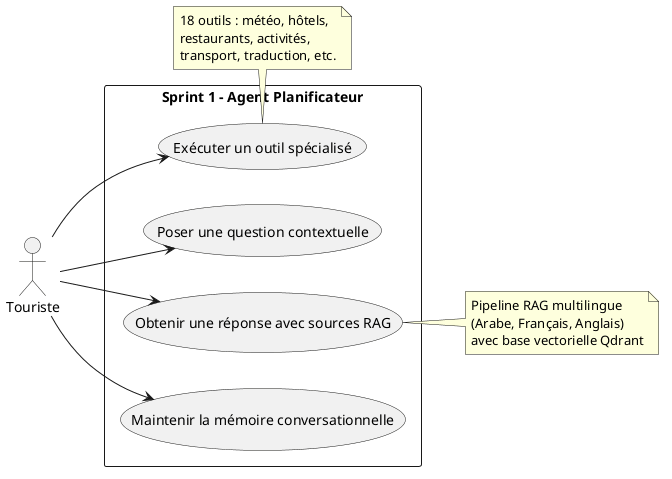
\includegraphics[width=0.85\textwidth]{diagrams/plantuml/usecase_sprint1.png}
    \caption{Diagramme de cas d'utilisation --- Sprint~1}
    \label{fig:uc_sprint1}
\end{figure}

\subsection{Description textuelle des cas d'utilisation}

\begin{table}[H]
    \centering
    \caption{Description textuelle --- CU : Envoyer un message au chatbot}
    \label{tab:cu_sprint1_1}
    \small
    \begin{tabular}{p{3cm} p{10cm}}
        \toprule
        \textbf{Champ} & \textbf{Description} \\
        \midrule
        Titre & Envoyer un message au chatbot \\[3pt]
        Acteur & Touriste \\[3pt]
        Pré-condition & L'utilisateur est connecté, une conversation est créée \\[3pt]
        Scénario nominal &
        1. L'utilisateur saisit un message dans l'interface de chat \newline
        2. Le frontend envoie la requête \texttt{POST /chat} au backend \newline
        3. Le backend vérifie l'existence de l'utilisateur en base \newline
        4. Le message est sauvegardé dans \texttt{PlannerMessage} \newline
        5. La réponse est retournée et affichée dans l'interface \\[3pt]
        Post-condition & Le message et la réponse sont persistés en base de données \\
        \bottomrule
    \end{tabular}
\end{table}

\begin{table}[H]
    \centering
    \caption{Description textuelle --- CU : Consulter l'historique des conversations}
    \label{tab:cu_sprint1_2}
    \small
    \begin{tabular}{p{3cm} p{10cm}}
        \toprule
        \textbf{Champ} & \textbf{Description} \\
        \midrule
        Titre & Consulter l'historique des conversations \\[3pt]
        Acteur & Touriste \\[3pt]
        Pré-condition & L'utilisateur est connecté et a au moins une conversation \\[3pt]
        Scénario nominal &
        1. L'utilisateur accède à la page d'historique \newline
        2. Le frontend envoie \texttt{GET /conversations/\{user\_id\}} \newline
        3. La liste des conversations est affichée avec date et résumé \newline
        4. L'utilisateur sélectionne une conversation pour voir les messages \\[3pt]
        Post-condition & Les messages de la conversation sélectionnée sont affichés \\
        \bottomrule
    \end{tabular}
\end{table}


% ────────────────────────────────────────────────────────────────
\section{Conception}
% ────────────────────────────────────────────────────────────────

\subsection{Diagramme de séquence --- Envoi d'un message}

Le diagramme de séquence suivant illustre le flux d'exécution lors de l'envoi d'un message
par le touriste au chatbot, de la saisie à l'affichage de la réponse.

\begin{figure}[H]
    \centering
    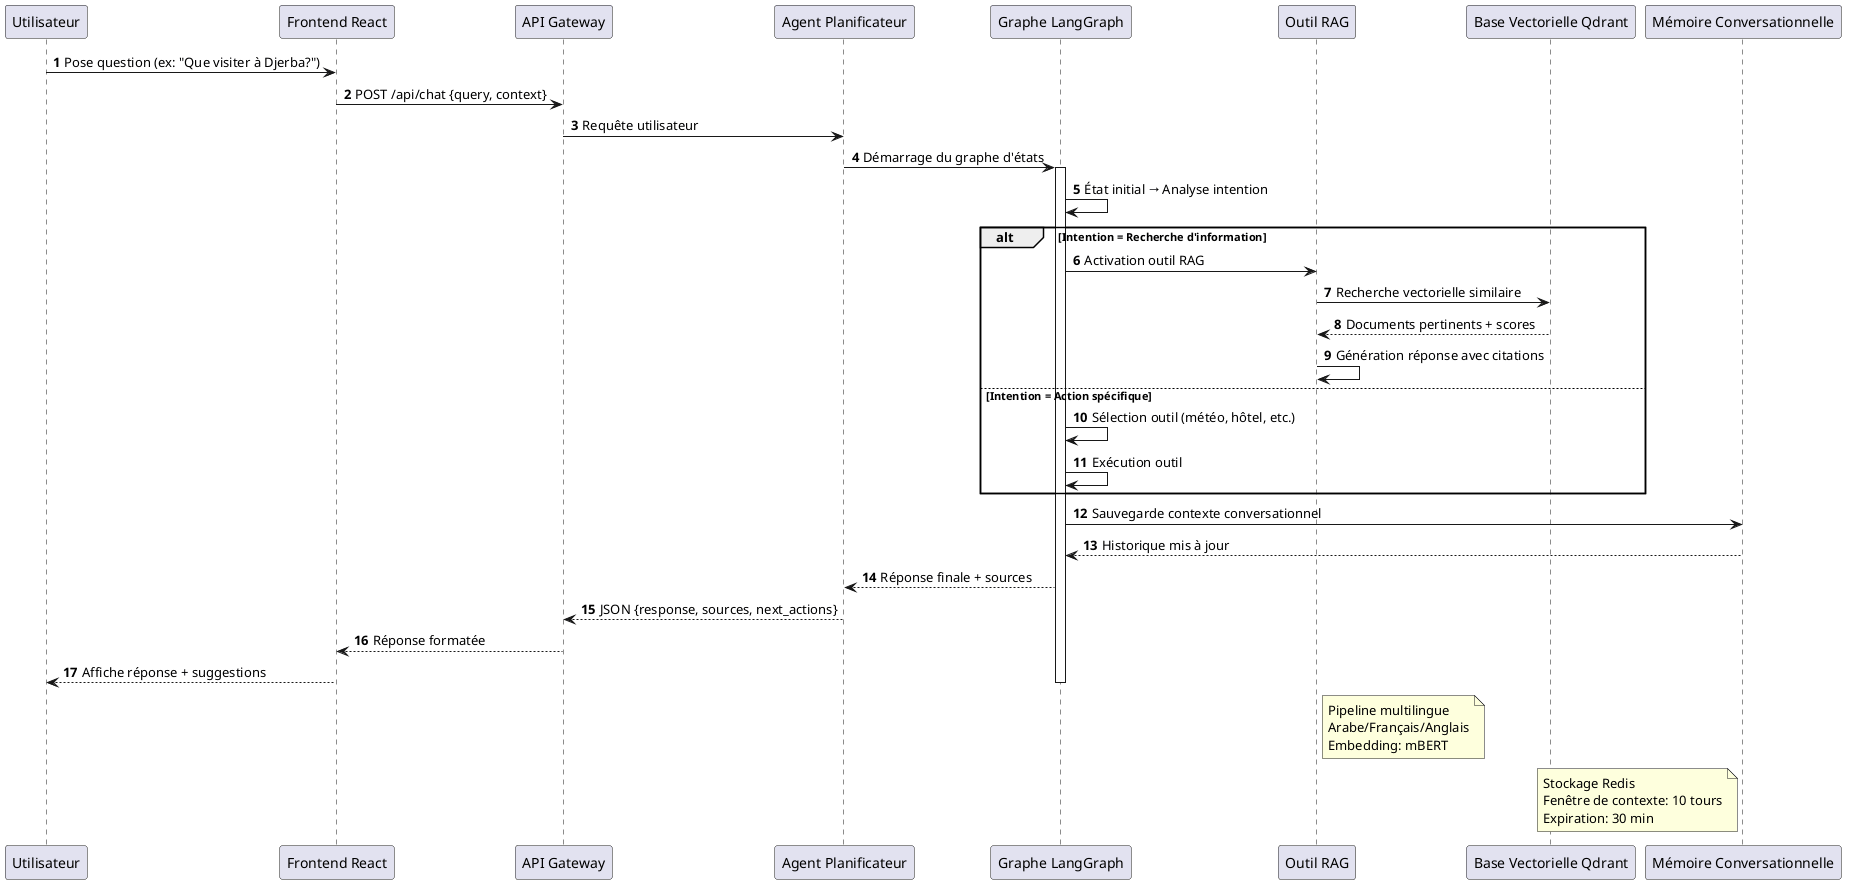
\includegraphics[width=\textwidth]{diagrams/plantuml/sequence_sprint1_primary.png}
    \caption{Diagramme de séquence --- Envoi d'un message au chatbot}
    \label{fig:seq_sprint1_primary}
\end{figure}

\subsection{Diagramme de séquence --- Consultation de l'historique}

\begin{figure}[H]
    \centering
    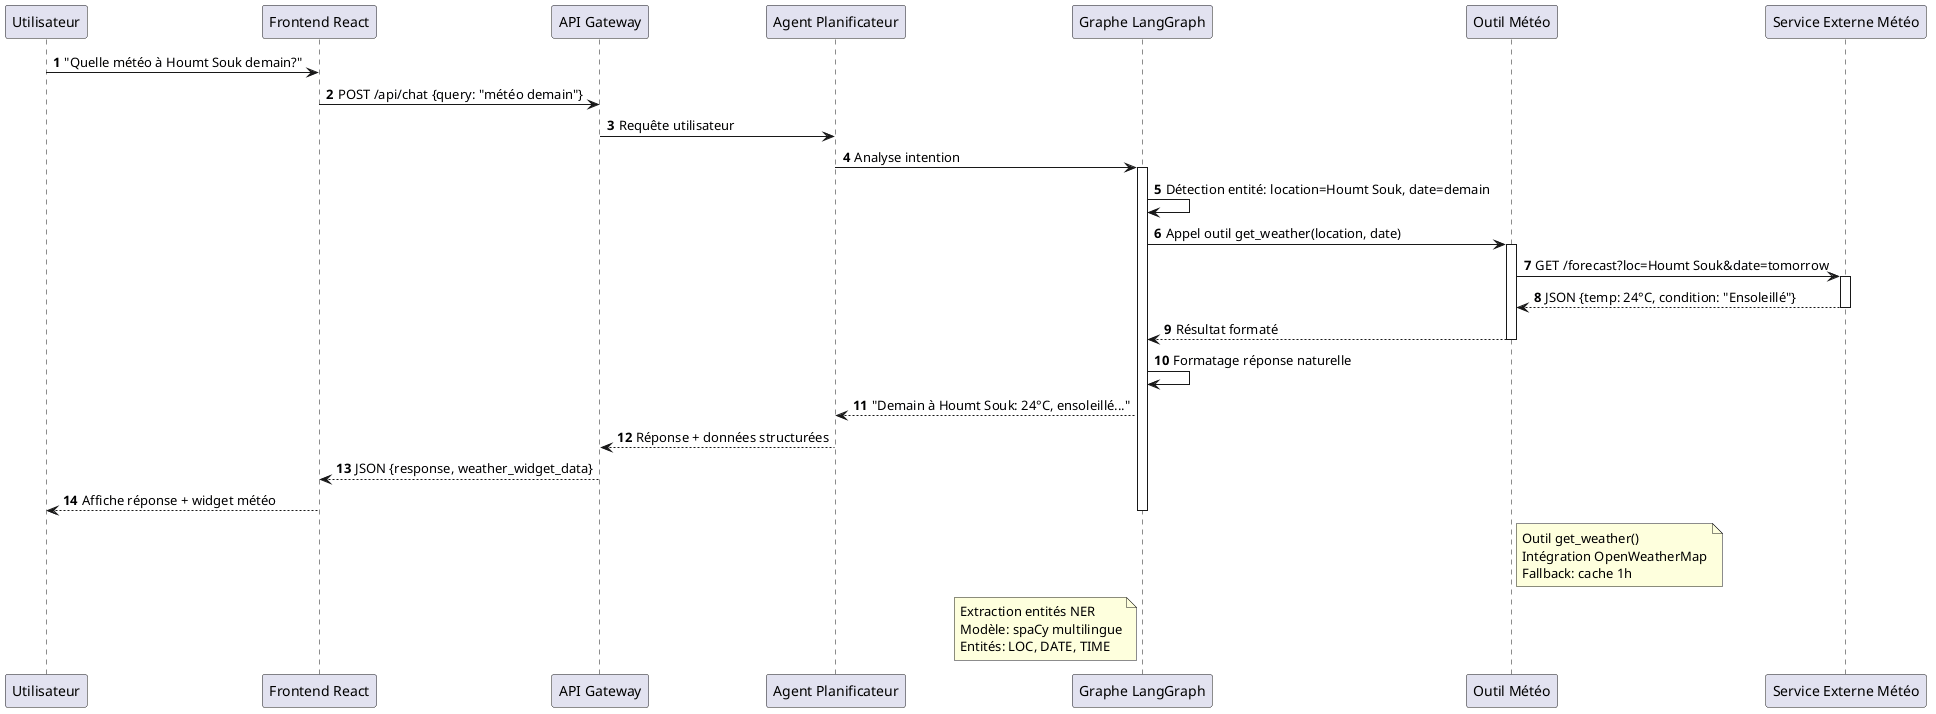
\includegraphics[width=\textwidth]{diagrams/plantuml/sequence_sprint1_secondary.png}
    \caption{Diagramme de séquence --- Consultation de l'historique des conversations}
    \label{fig:seq_sprint1_secondary}
\end{figure}


% ────────────────────────────────────────────────────────────────
\section{Réalisation}
% ────────────────────────────────────────────────────────────────

\subsection{Structure du projet}

L'environnement de développement a été mis en place avec la structure suivante~:
\begin{itemize}
    \item \texttt{planner-agent/app/}~: code source du backend IA (FastAPI)
    \item \texttt{planner-agent/app/reco/}~: module de recommandation LinUCB
    \item \texttt{src/}~: code source du frontend Next.js / Prisma
    \item \texttt{prisma/schema.prisma}~: modèle de données du frontend
\end{itemize}

Les technologies suivantes ont été installées et configurées~: Python 3.12, FastAPI,
SQLAlchemy (mode asynchrone avec asyncpg), PostgreSQL 15, Ollama avec le modèle qwen2.5:7b,
et Next.js pour le frontend.

\subsection{Interface de chat}

L'interface de chat a été intégrée dans le frontend Next.js. Elle permet au touriste de
formuler des requêtes en langage naturel et d'afficher les réponses de l'agent en temps réel
grâce au streaming.

\begin{figure}[H]
    \centering
    
\includegraphics[width=\textwidth]{diagrams/screen_A4_chat_interface.png}
    \caption{Interface de chat de la plateforme Guidni}
    \label{fig:screen_chat}
\end{figure}

\subsection{Base de données}

Les tables du sous-système planificateur (\texttt{PlannerConversation}, \texttt{PlannerMessage},
\texttt{GeneratedPlan}, \texttt{ActivityIntelligence}) et du sous-système recommandation
(\texttt{BanditArm}, \texttt{LinUCBGlobal}, \texttt{UserProfile}, \texttt{UserSession},
\texttt{RecommendationEvent}, \texttt{ListingTag}, \texttt{SystemConfig}) ont été créées.

\begin{figure}[H]
    \centering
    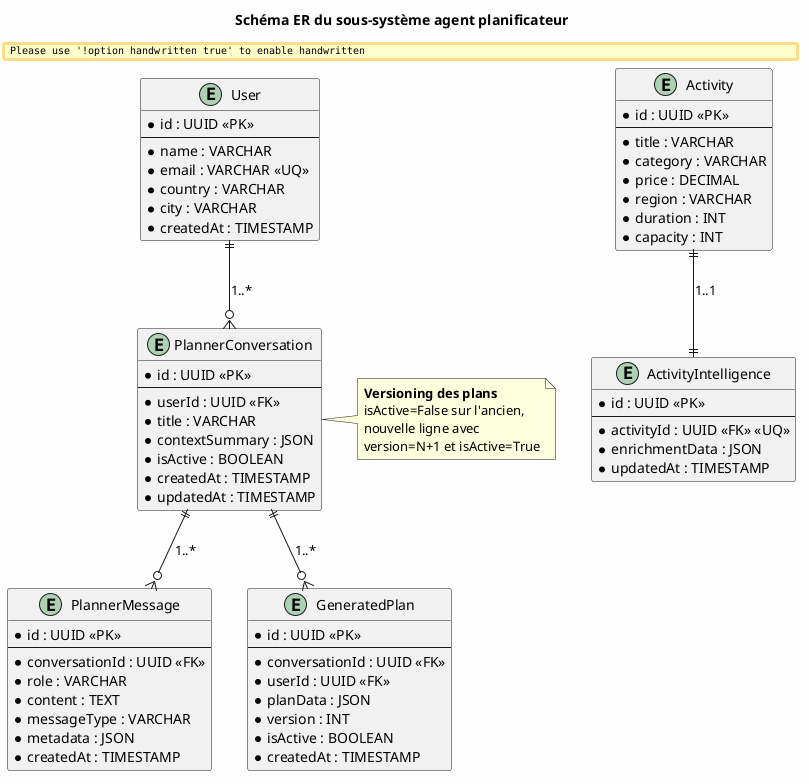
\includegraphics[width=\textwidth]{diagrams/fig_03_er_diagram_planner.png}
    \caption{Aperçu du schéma de la base de données dans pgAdmin}
    \label{fig:screen_db}
\end{figure}

\subsection{Documentation API}

La documentation OpenAPI a été générée automatiquement par FastAPI et est accessible via
l'endpoint \texttt{/docs}. Elle décrit les 12~endpoints du système avec leurs schémas de
requête et de réponse.

\begin{figure}[H]
    \centering
    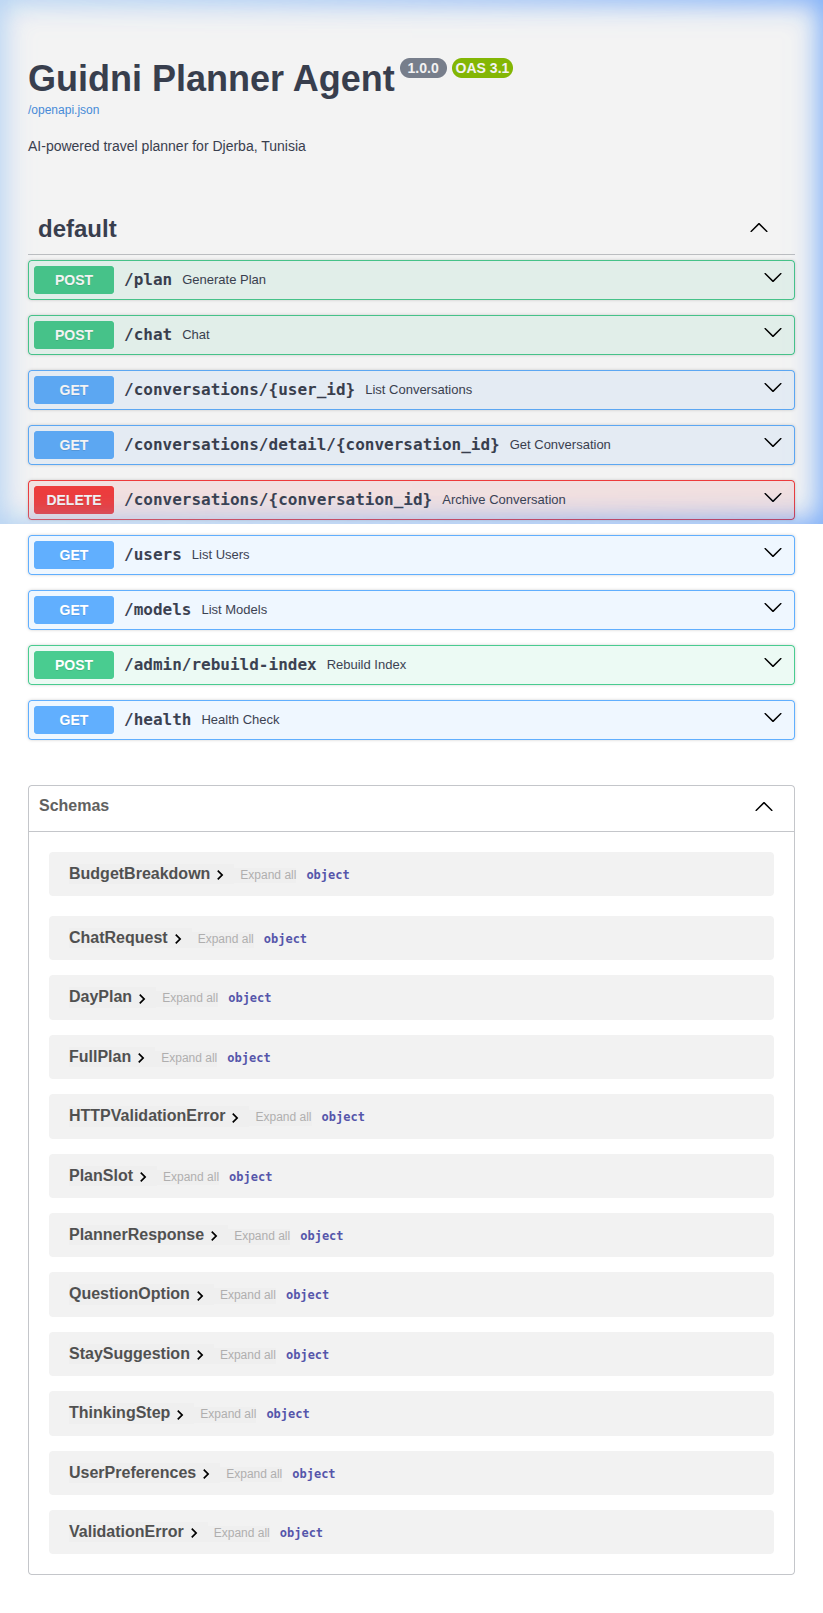
\includegraphics[width=\textwidth]{diagrams/screen_A4_api_docs.png}
    \caption{Documentation OpenAPI générée par FastAPI}
    \label{fig:screen_api}
\end{figure}

\subsection{Health check et supervision}

L'endpoint \texttt{GET /health} permet de vérifier l'état de santé du système en temps réel,
incluant la connectivité base de données, la disponibilité du modèle LLM et l'état de l'index
vectoriel.

\begin{figure}[H]
    \centering
    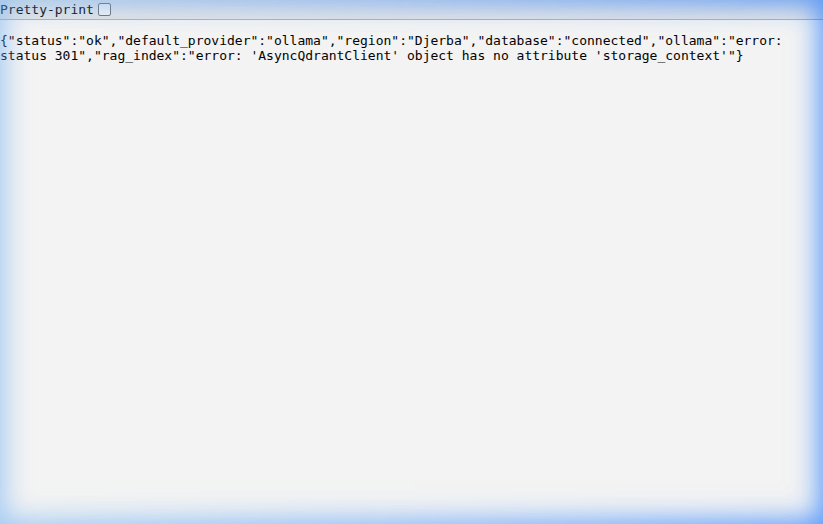
\includegraphics[width=\textwidth]{diagrams/screen_A4_health_check.png}
    \caption{Endpoint de health check du système Guidni}
    \label{fig:screen_health}
\end{figure}

\subsection{Schéma de la base de données -- Recommandation}

En parallèle du schéma planificateur, les tables du sous-système de recommandation ont été
créées pour préparer le Sprint~4.

\begin{figure}[H]
    \centering
    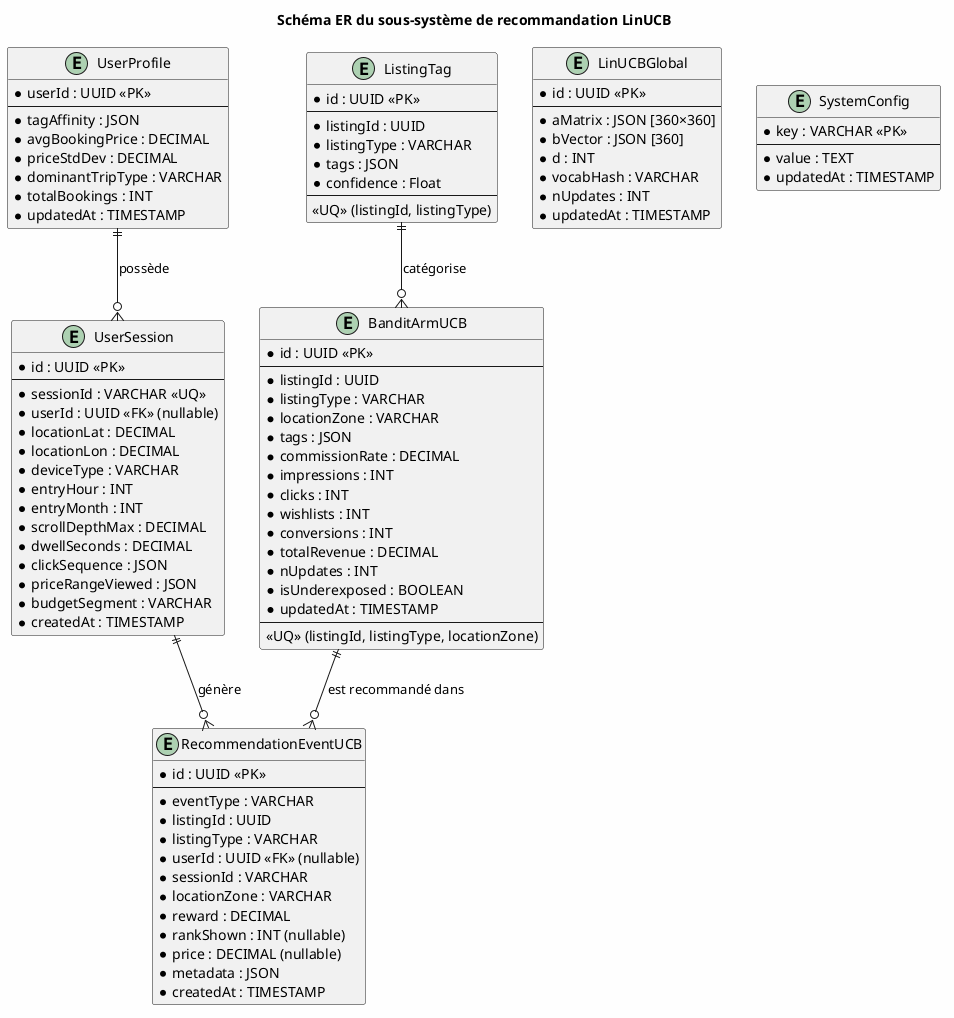
\includegraphics[width=\textwidth]{diagrams/fig_03_er_diagram_recommender.png}
    \caption{Schéma ER du sous-système de recommandation}
    \label{fig:screen_er_reco}
\end{figure}


% ────────────────────────────────────────────────────────────────
\section{Sprint Review}
% ────────────────────────────────────────────────────────────────

À la clôture du Sprint~1, la phase de Sprint Review s'est tenue en présence de l'encadrant
M.~Nizar Tenzekhti. Les éléments suivants ont été validés~:
\begin{itemize}
    \item L'environnement de développement est opérationnel.
    \item Les schémas de base de données sont créés et migrés.
    \item L'interface de chat est connectée au backend et affiche les messages.
    \item La documentation API est générée et accessible.
\end{itemize}

Lors de la Sprint Retrospective, l'encadrant a formellement approuvé l'architecture proposée
et a souligné l'importance de documenter rigoureusement les flux asynchrones entre les appels
base de données et les API des grands modèles de langage.


% ────────────────────────────────────────────────────────────────
\section*{Conclusion}
\addcontentsline{toc}{section}{Conclusion}

Le Sprint~1 a permis de poser les fondations du projet Guidni. L'environnement de
développement a été configuré, les schémas de base de données ont été conçus et migrés,
les contrats API REST ont été formalisés, et l'interface de chat a été intégrée au frontend.
Ces bases solides permettront d'aborder le Sprint~2 avec confiance, qui sera consacré à
l'implémentation du pipeline RAG multilingue et de la recherche sémantique.
